\subsection{Resultatbehandling af det udvidede problem} \label{kap:resultat_udvidet}

Vi kigger i dette afsnit på de resultater, vores algoritme har fundet i det udvidede problem. Den længste vej er fundet ved brug af vores korteste vej-algoritme med fremgangsmåden, som er gennemgået i \autoref{kap:grafen_for_udvidet}. På \autoref{fig:gaslager_graf_udvidet} kan man se den længste vej igennem grafen for det udvidede problem.
\begin{figure}[H]
\centering
	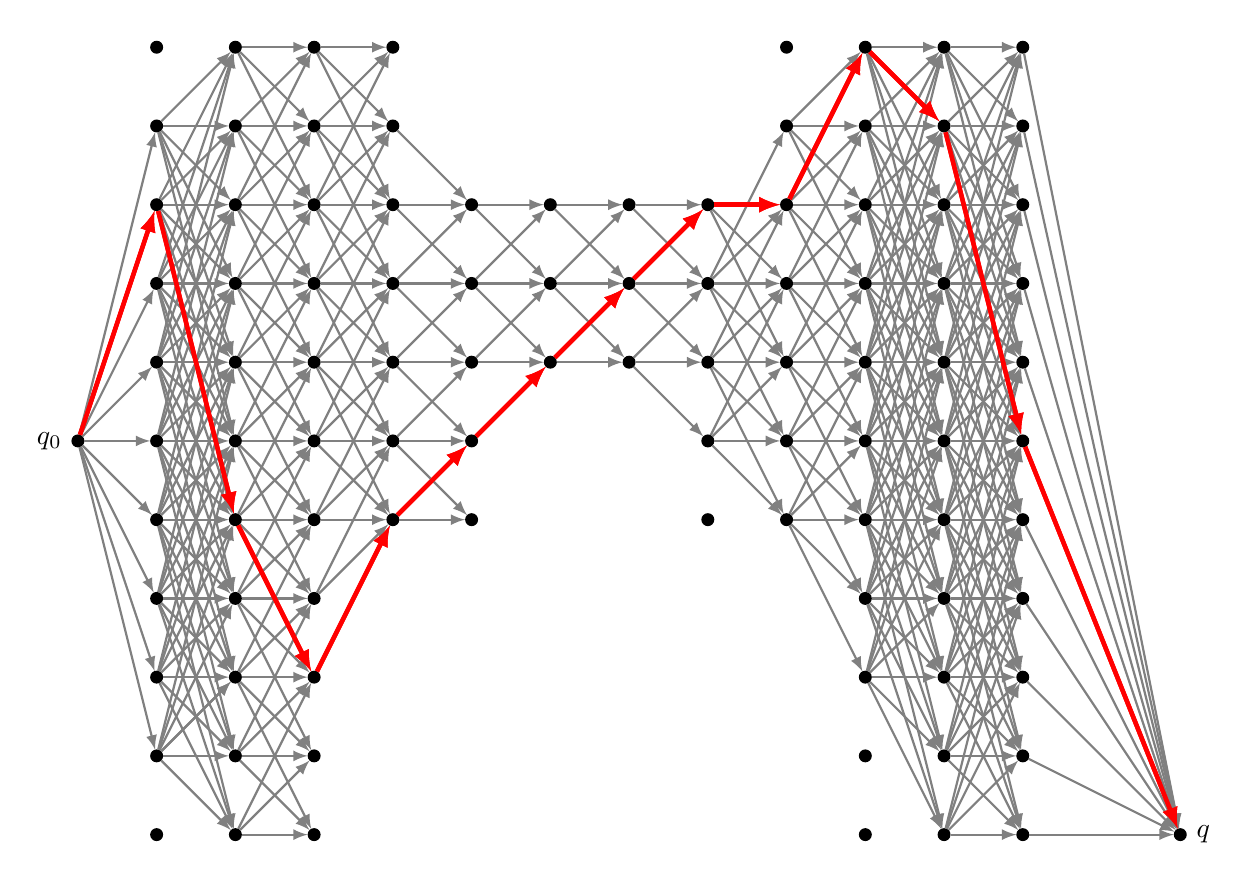
\begin{tikzpicture}

       \tikzset{enclosed/.style={draw, circle, inner sep=0pt, minimum size=.15cm, fill=black}}
%% Vertices
      	\node[enclosed, label={left: $q_{0}$}] (vstart) at (-1,5) {};
      	\node[enclosed, label={below: }] (v00) at (0,0) {};
    		\node[enclosed, label={below: }] (v01) at (0,1) {};
  	    \node[enclosed, label={above: }] (v02) at (0,2) {};
     	\node[enclosed, label={below: }] (v03) at (0,3) {};
     	\node[enclosed, label={below:  }] (v04) at (0,4) {};
     	\node[enclosed, label={above: }] (v05) at (0,5) {};
     	\node[enclosed, label={below: }] (v06) at (0,6) {};
     	\node[enclosed, label={below: }] (v07) at (0,7) {};
     	\node[enclosed, label={above: }] (v08) at (0,8) {};
     	\node[enclosed, label={below:  }] (v09) at (0,9) {};
     	\node[enclosed, label={below: }] (v010) at (0,10) {};
      	\node[enclosed, label={above: }] (v10) at (1,0) {};
  	    \node[enclosed, label={below: }] (v11) at (1,1) {};
  	    \node[enclosed, label={below: }] (v12) at (1,2) {};
     	\node[enclosed, label={above:  }] (v13) at (1,3) {};
     	\node[enclosed, label={below: }] (v14) at (1,4) {};
     	 \node[enclosed, label={below:}] (v15) at (1,5) {};
     	\node[enclosed, label={above: }] (v16) at (1,6) {};
     	\node[enclosed, label={below: }] (v17) at (1,7) {};
     	\node[enclosed, label={above: }] (v18) at (1,8) {};
     	\node[enclosed, label={below:  }] (v19) at (1,9) {};
     	\node[enclosed, label={below: }] (v110) at (1,10) {};
     	\node[enclosed, label={below: }] (v20) at (2,0) {};
    		\node[enclosed, label={below: }] (v21) at (2,1) {};
  	    \node[enclosed, label={above: }] (v22) at (2,2) {};
     	\node[enclosed, label={below: }] (v23) at (2,3) {};
     	\node[enclosed, label={below:  }] (v24) at (2,4) {};
     	\node[enclosed, label={above: }] (v25) at (2,5) {};
     	\node[enclosed, label={below: }] (v26) at (2,6) {};
     	\node[enclosed, label={below: }] (v27) at (2,7) {};
     	\node[enclosed, label={above: }] (v28) at (2,8) {};
     	\node[enclosed, label={below:  }] (v29) at (2,9) {};
     	\node[enclosed, label={below: }] (v210) at (2,10) {};
     	\node[enclosed, label={below: }] (v34) at (3,4) {};
     	 \node[enclosed, label={below:}] (v35) at (3,5) {};
     	\node[enclosed, label={above: }] (v36) at (3,6) {};
     	\node[enclosed, label={below: }] (v37) at (3,7) {};
     	\node[enclosed, label={above: }] (v38) at (3,8) {};
     	\node[enclosed, label={below:  }] (v39) at (3,9) {};
     	\node[enclosed, label={below: }] (v310) at (3,10) {};
     	\node[enclosed, label={below:  }] (v44) at (4,4) {};
     	\node[enclosed, label={above: }] (v45) at (4,5) {};
     	\node[enclosed, label={below: }] (v46) at (4,6) {};
     	\node[enclosed, label={below: }] (v47) at (4,7) {};
     	\node[enclosed, label={above: }] (v48) at (4,8) {};
     	\node[enclosed, label={above: }] (v56) at (5,6) {};
     	\node[enclosed, label={below: }] (v57) at (5,7) {};
     	\node[enclosed, label={above: }] (v58) at (5,8) {};
     	\node[enclosed, label={below: }] (v66) at (6,6) {};
     	\node[enclosed, label={below: }] (v67) at (6,7) {};
     	\node[enclosed, label={above: }] (v68) at (6,8) {};
     	\node[enclosed, label={below: }] (v74) at (7,4) {};
     	 \node[enclosed, label={below:}] (v75) at (7,5) {};
     	\node[enclosed, label={above: }] (v76) at (7,6) {};
     	\node[enclosed, label={below: }] (v77) at (7,7) {};
     	\node[enclosed, label={above: }] (v78) at (7,8) {};
     	\node[enclosed, label={below: }] (v84) at (8,4) {};
     	 \node[enclosed, label={below:}] (v85) at (8,5) {};
     	\node[enclosed, label={above: }] (v86) at (8,6) {};
     	\node[enclosed, label={below: }] (v87) at (8,7) {};
     	\node[enclosed, label={above: }] (v88) at (8,8) {};
     	\node[enclosed, label={below:  }] (v89) at (8,9) {};
     	\node[enclosed, label={below: }] (v810) at (8,10) {};
     	\node[enclosed, label={below: }] (v90) at (9,0) {};
    		\node[enclosed, label={below: }] (v91) at (9,1) {};
  	    \node[enclosed, label={above: }] (v92) at (9,2) {};
     	\node[enclosed, label={below: }] (v93) at (9,3) {};
     	\node[enclosed, label={below:  }] (v94) at (9,4) {};
     	\node[enclosed, label={above: }] (v95) at (9,5) {};
     	\node[enclosed, label={below: }] (v96) at (9,6) {};
     	\node[enclosed, label={below: }] (v97) at (9,7) {};
     	\node[enclosed, label={above: }] (v98) at (9,8) {};
     	\node[enclosed, label={below:  }] (v99) at (9,9) {};
     	\node[enclosed, label={below: }] (v910) at (9,10) {};
      	\node[enclosed, label={above: }] (v100) at (10,0) {};
  	    \node[enclosed, label={below: }] (v101) at (10,1) {};
  	    \node[enclosed, label={below: }] (v102) at (10,2) {};
     	\node[enclosed, label={above:  }] (v103) at (10,3) {};
     	\node[enclosed, label={below: }] (v104) at (10,4) {};
     	 \node[enclosed, label={below:}] (v105) at (10,5) {};
     	\node[enclosed, label={above: }] (v106) at (10,6) {};
     	\node[enclosed, label={below: }] (v107) at (10,7) {};
     	\node[enclosed, label={above: }] (v108) at (10,8) {};
     	\node[enclosed, label={below:  }] (v109) at (10,9) {};
     	\node[enclosed, label={below: }] (v1010) at (10,10) {};
     	\node[enclosed, label={above: }] (v1100) at (11,0) {};
  	    \node[enclosed, label={below: }] (v111) at (11,1) {};
  	    \node[enclosed, label={below: }] (v112) at (11,2) {};
     	\node[enclosed, label={above:  }] (v113) at (11,3) {};
     	\node[enclosed, label={below: }] (v114) at (11,4) {};
     	 \node[enclosed, label={below:}] (v115) at (11,5) {};
     	\node[enclosed, label={above: }] (v116) at (11,6) {};
     	\node[enclosed, label={below: }] (v117) at (11,7) {};
     	\node[enclosed, label={above: }] (v118) at (11,8) {};
     	\node[enclosed, label={below:  }] (v119) at (11,9) {};
     	\node[enclosed, label={below: }] (v1110) at (11,10) {};
     	\node[enclosed, label={right: $q_{\slut}$ }] (v120) at (13,0) {};
     	
%Edges
		\path[gray,->,>=latex,thick] (vstart) edge node[midway, sloped, above] {} (v01);
		\path[gray,->,>=latex,thick] (vstart) edge node[midway, sloped, below] {} (v02);
		\path[gray,->,>=latex,thick] (vstart) edge node[midway, sloped, below] {} (v03);
		\path[gray,->,>=latex,thick] (vstart) edge node[midway, sloped, above] {} (v04);
		\path[gray,->,>=latex,thick] (vstart) edge node[midway, above] {} (v05);
		\path[gray,->,>=latex,thick] (vstart) edge node[near end, sloped, below] {} (v06);
		\path[gray,->,>=latex,thick] (vstart) edge node[midway, sloped, below] {} (v07);
		\path[red,->,>=latex,ultra thick] (vstart) edge node[midway, above] {} (v08);
		\path[gray,->,>=latex,thick] (vstart) edge node[near end, sloped, below] {} (v09);
		\path[gray,->,>=latex,thick] (v01) edge node[midway, sloped, below] {} (v10);
		\path[gray,->,>=latex,thick] (v01) edge node[midway, sloped, above] {} (v11);
		\path[gray,->,>=latex,thick] (v01) edge node[midway, above] {} (v12);
		\path[gray,->,>=latex,thick] (v01) edge node[near end, sloped, below] {} (v12);
		\path[gray,->,>=latex,thick] (v01) edge node[midway, sloped, below] {} (v13);
		\path[gray,->,>=latex,thick] (v01) edge node[midway, above] {} (v14);
		\path[gray,->,>=latex,thick] (v01) edge node[near end, sloped, below] {} (v15);
		\path[gray,->,>=latex,thick] (v02) edge node[midway, sloped, below] {} (v10);
		\path[gray,->,>=latex,thick] (v02) edge node[midway, sloped, above] {} (v11);
		\path[gray,->,>=latex,thick] (v02) edge node[midway, above] {} (v12);
		\path[gray,->,>=latex,thick] (v02) edge node[near end, sloped, below] {} (v13);
		\path[gray,->,>=latex,thick] (v02) edge node[midway, sloped, below] {} (v14);
		\path[gray,->,>=latex,thick] (v02) edge node[midway, above] {} (v15);
		\path[gray,->,>=latex,thick] (v02) edge node[near end, sloped, below] {} (v16);
		\path[gray,->,>=latex,thick] (v03) edge node[midway, sloped, below] {} (v10);
		\path[gray,->,>=latex,thick] (v03) edge node[midway, sloped, above] {} (v11);
		\path[gray,->,>=latex,thick] (v03) edge node[midway, above] {} (v12);
		\path[gray,->,>=latex,thick] (v03) edge node[near end, sloped, below] {} (v13);
		\path[gray,->,>=latex,thick] (v03) edge node[midway, sloped, below] {} (v14);
		\path[gray,->,>=latex,thick] (v03) edge node[midway, above] {} (v15);
		\path[gray,->,>=latex,thick] (v03) edge node[near end, sloped, below] {} (v16);
		\path[gray,->,>=latex,thick] (v03) edge node[midway, sloped, below] {} (v17);
		\path[gray,->,>=latex,thick] (v04) edge node[midway, sloped, below] {} (v10);
		\path[gray,->,>=latex,thick] (v04) edge node[midway, sloped, above] {} (v11);
		\path[gray,->,>=latex,thick] (v04) edge node[midway, above] {} (v12);
		\path[gray,->,>=latex,thick] (v04) edge node[near end, sloped, below] {} (v13);
		\path[gray,->,>=latex,thick] (v04) edge node[midway, sloped, below] {} (v14);
		\path[gray,->,>=latex,thick] (v04) edge node[midway, above] {} (v15);
		\path[gray,->,>=latex,thick] (v04) edge node[near end, sloped, below] {} (v16);
		\path[gray,->,>=latex,thick] (v04) edge node[midway, sloped, below] {} (v17);
		\path[gray,->,>=latex,thick] (v04) edge node[midway, sloped, above] {} (v18);
		\path[gray,->,>=latex,thick] (v05) edge node[midway, sloped, above] {} (v11);
		\path[gray,->,>=latex,thick] (v05) edge node[midway, above] {} (v12);
		\path[gray,->,>=latex,thick] (v05) edge node[near end, sloped, below] {} (v13);
		\path[gray,->,>=latex,thick] (v05) edge node[midway, sloped, below] {} (v14);
		\path[gray,->,>=latex,thick] (v05) edge node[midway, above] {} (v15);
		\path[gray,->,>=latex,thick] (v05) edge node[near end, sloped, below] {} (v16);
		\path[gray,->,>=latex,thick] (v05) edge node[midway, sloped, below] {} (v17);
		\path[gray,->,>=latex,thick] (v05) edge node[midway, sloped, above] {} (v18);
		\path[gray,->,>=latex,thick] (v05) edge node[midway, sloped, above] {} (v19);
		\path[gray,->,>=latex,thick] (v06) edge node[midway, above] {} (v12);
		\path[gray,->,>=latex,thick] (v06) edge node[near end, sloped, below] {} (v13);
		\path[gray,->,>=latex,thick] (v06) edge node[midway, sloped, below] {} (v14);
		\path[gray,->,>=latex,thick] (v06) edge node[midway, above] {} (v15);
		\path[gray,->,>=latex,thick] (v06) edge node[near end, sloped, below] {} (v16);
		\path[gray,->,>=latex,thick] (v06) edge node[midway, sloped, below] {} (v17);
		\path[gray,->,>=latex,thick] (v06) edge node[midway, sloped, above] {} (v18);
		\path[gray,->,>=latex,thick] (v06) edge node[midway, sloped, above] {} (v19);
		\path[gray,->,>=latex,thick] (v06) edge node[midway, sloped, above] {} (v110);
		\path[gray,->,>=latex,thick] (v07) edge node[near end, sloped, below] {} (v13);
		\path[gray,->,>=latex,thick] (v07) edge node[midway, sloped, below] {} (v14);
		\path[gray,->,>=latex,thick] (v07) edge node[midway, above] {} (v15);
		\path[gray,->,>=latex,thick] (v07) edge node[near end, sloped, below] {} (v16);
		\path[gray,->,>=latex,thick] (v07) edge node[midway, sloped, below] {} (v17);
		\path[gray,->,>=latex,thick] (v07) edge node[midway, sloped, above] {} (v18);
		\path[gray,->,>=latex,thick] (v07) edge node[midway, sloped, above] {} (v19);
		\path[gray,->,>=latex,thick] (v07) edge node[midway, sloped, above] {} (v110);
		\path[red,->,>=latex,ultra thick] (v08) edge node[midway, sloped, below] {} (v14);
		\path[gray,->,>=latex,thick] (v08) edge node[midway, above] {} (v15);
		\path[gray,->,>=latex,thick] (v08) edge node[near end, sloped, below] {} (v16);
		\path[gray,->,>=latex,thick] (v08) edge node[midway, sloped, below] {} (v17);
		\path[gray,->,>=latex,thick] (v08) edge node[midway, sloped, above] {} (v18);
		\path[gray,->,>=latex,thick] (v08) edge node[midway, sloped, above] {} (v19);
		\path[gray,->,>=latex,thick] (v08) edge node[midway, sloped, above] {} (v110);
		\path[gray,->,>=latex,thick] (v09) edge node[midway, above] {} (v15);
		\path[gray,->,>=latex,thick] (v09) edge node[near end, sloped, below] {} (v16);
		\path[gray,->,>=latex,thick] (v09) edge node[midway, sloped, below] {} (v17);
		\path[gray,->,>=latex,thick] (v09) edge node[midway, sloped, above] {} (v18);
		\path[gray,->,>=latex,thick] (v09) edge node[midway, sloped, above] {} (v19);
		\path[gray,->,>=latex,thick] (v09) edge node[midway, sloped, above] {} (v110);
		\path[gray,->,>=latex,thick] (v10) edge node[midway, sloped, below] {} (v20);
		\path[gray,->,>=latex,thick] (v10) edge node[midway, sloped, above] {} (v21);
		\path[gray,->,>=latex,thick] (v10) edge node[midway, above] {} (v22);
		\path[gray,->,>=latex,thick] (v11) edge node[midway, sloped, below] {} (v20);
		\path[gray,->,>=latex,thick] (v11) edge node[midway, sloped, above] {} (v21);
		\path[gray,->,>=latex,thick] (v11) edge node[midway, above] {} (v22);
		\path[gray,->,>=latex,thick] (v11) edge node[midway, sloped, below] {} (v23);
		\path[gray,->,>=latex,thick] (v12) edge node[midway, sloped, below] {} (v20);
		\path[gray,->,>=latex,thick] (v12) edge node[midway, sloped, above] {} (v21);
		\path[gray,->,>=latex,thick] (v12) edge node[midway, above] {} (v22);
		\path[gray,->,>=latex,thick] (v12) edge node[near end, sloped, below] {} (v23);
		\path[gray,->,>=latex,thick] (v12) edge node[midway, sloped, below] {} (v24);
		\path[gray,->,>=latex,thick] (v13) edge node[midway, sloped, above] {} (v21);
		\path[gray,->,>=latex,thick] (v13) edge node[midway, above] {} (v22);
		\path[gray,->,>=latex,thick] (v13) edge node[near end, sloped, below] {} (v23);
		\path[gray,->,>=latex,thick] (v13) edge node[midway, sloped, below] {} (v24);
		\path[gray,->,>=latex,thick] (v13) edge node[midway, above] {} (v25);
		\path[red,->,>=latex,ultra thick] (v14) edge node[midway, above] {} (v22);
		\path[gray,->,>=latex,thick] (v14) edge node[near end, sloped, below] {} (v23);
		\path[gray,->,>=latex,thick] (v14) edge node[midway, sloped, below] {} (v24);
		\path[gray,->,>=latex,thick] (v14) edge node[midway, above] {} (v25);
		\path[gray,->,>=latex,thick] (v14) edge node[near end, sloped, below] {} (v26);
		\path[gray,->,>=latex,thick] (v15) edge node[near end, sloped, below] {} (v23);
		\path[gray,->,>=latex,thick] (v15) edge node[midway, sloped, below] {} (v24);
		\path[gray,->,>=latex,thick] (v15) edge node[midway, above] {} (v25);
		\path[gray,->,>=latex,thick] (v15) edge node[near end, sloped, below] {} (v26);
		\path[gray,->,>=latex,thick] (v15) edge node[midway, sloped, below] {} (v27);
		\path[gray,->,>=latex,thick] (v16) edge node[midway, sloped, below] {} (v24);
		\path[gray,->,>=latex,thick] (v16) edge node[midway, above] {} (v25);
		\path[gray,->,>=latex,thick] (v16) edge node[near end, sloped, below] {} (v26);
		\path[gray,->,>=latex,thick] (v16) edge node[midway, sloped, below] {} (v27);
		\path[gray,->,>=latex,thick] (v16) edge node[midway, sloped, above] {} (v28);
		\path[gray,->,>=latex,thick] (v17) edge node[midway, above] {} (v25);
		\path[gray,->,>=latex,thick] (v17) edge node[near end, sloped, below] {} (v26);
		\path[gray,->,>=latex,thick] (v17) edge node[midway, sloped, below] {} (v27);
		\path[gray,->,>=latex,thick] (v17) edge node[midway, sloped, above] {} (v28);
		\path[gray,->,>=latex,thick] (v17) edge node[midway, sloped, above] {} (v29);
		\path[gray,->,>=latex,thick] (v18) edge node[near end, sloped, below] {} (v26);
		\path[gray,->,>=latex,thick] (v18) edge node[midway, sloped, below] {} (v27);
		\path[gray,->,>=latex,thick] (v18) edge node[midway, sloped, above] {} (v28);
		\path[gray,->,>=latex,thick] (v18) edge node[midway, sloped, above] {} (v29);
		\path[gray,->,>=latex,thick] (v18) edge node[midway, sloped, above] {} (v210);
		\path[gray,->,>=latex,thick] (v19) edge node[midway, sloped, below] {} (v27);
		\path[gray,->,>=latex,thick] (v19) edge node[midway, sloped, above] {} (v28);
		\path[gray,->,>=latex,thick] (v19) edge node[midway, sloped, above] {} (v29);
		\path[gray,->,>=latex,thick] (v19) edge node[midway, sloped, above] {} (v210);
		\path[gray,->,>=latex,thick] (v110) edge node[midway, sloped, above] {} (v28);
		\path[gray,->,>=latex,thick] (v110) edge node[midway, sloped, above] {} (v29);
		\path[gray,->,>=latex,thick] (v110) edge node[midway, sloped, above] {} (v210);
		\path[red,->,>=latex,ultra thick] (v22) edge node[midway, sloped, below] {} (v34);
		\path[gray,->,>=latex,thick] (v23) edge node[midway, sloped, below] {} (v34);
		\path[gray,->,>=latex,thick] (v23) edge node[midway, above] {} (v35);
		\path[gray,->,>=latex,thick] (v24) edge node[midway, sloped, below] {} (v34);
		\path[gray,->,>=latex,thick] (v24) edge node[midway, above] {} (v35);
		\path[gray,->,>=latex,thick] (v24) edge node[near end, sloped, below] {} (v36);
		\path[gray,->,>=latex,thick] (v25) edge node[midway, sloped, below] {} (v34);
		\path[gray,->,>=latex,thick] (v25) edge node[midway, above] {} (v35);
		\path[gray,->,>=latex,thick] (v25) edge node[near end, sloped, below] {} (v36);
		\path[gray,->,>=latex,thick] (v25) edge node[midway, sloped, below] {} (v37);
		\path[gray,->,>=latex,thick] (v26) edge node[midway, sloped, below] {} (v34);
		\path[gray,->,>=latex,thick] (v26) edge node[midway, above] {} (v35);
		\path[gray,->,>=latex,thick] (v26) edge node[near end, sloped, below] {} (v36);
		\path[gray,->,>=latex,thick] (v26) edge node[midway, sloped, below] {} (v37);
		\path[gray,->,>=latex,thick] (v26) edge node[midway, sloped, above] {} (v38);
		\path[gray,->,>=latex,thick] (v27) edge node[midway, above] {} (v35);
		\path[gray,->,>=latex,thick] (v27) edge node[near end, sloped, below] {} (v36);
		\path[gray,->,>=latex,thick] (v27) edge node[midway, sloped, below] {} (v37);
		\path[gray,->,>=latex,thick] (v27) edge node[midway, sloped, above] {} (v38);
		\path[gray,->,>=latex,thick] (v27) edge node[midway, sloped, above] {} (v39);
		\path[gray,->,>=latex,thick] (v28) edge node[near end, sloped, below] {} (v36);
		\path[gray,->,>=latex,thick] (v28) edge node[midway, sloped, below] {} (v37);
		\path[gray,->,>=latex,thick] (v28) edge node[midway, sloped, above] {} (v38);
		\path[gray,->,>=latex,thick] (v28) edge node[midway, sloped, above] {} (v39);
		\path[gray,->,>=latex,thick] (v28) edge node[midway, sloped, above] {} (v310);
		\path[gray,->,>=latex,thick] (v29) edge node[midway, sloped, below] {} (v37);
		\path[gray,->,>=latex,thick] (v29) edge node[midway, sloped, above] {} (v38);
		\path[gray,->,>=latex,thick] (v29) edge node[midway, sloped, above] {} (v39);
		\path[gray,->,>=latex,thick] (v29) edge node[midway, sloped, above] {} (v310);
		\path[gray,->,>=latex,thick] (v210) edge node[midway, sloped, above] {} (v38);
		\path[gray,->,>=latex,thick] (v210) edge node[midway, sloped, above] {} (v39);
		\path[gray,->,>=latex,thick] (v210) edge node[midway, sloped, above] {} (v310);
		\path[gray,->,>=latex,thick] (v34) edge node[midway, sloped, below] {} (v44);
		\path[red,->,>=latex,ultra thick] (v34) edge node[midway, above] {} (v45);
		\path[gray,->,>=latex,thick] (v35) edge node[midway, sloped, below] {} (v44);
		\path[gray,->,>=latex,thick] (v35) edge node[midway, above] {} (v45);
		\path[gray,->,>=latex,thick] (v35) edge node[near end, sloped, below] {} (v46);
		\path[gray,->,>=latex,thick] (v36) edge node[midway, above] {} (v45);
		\path[gray,->,>=latex,thick] (v36) edge node[near end, sloped, below] {} (v46);
		\path[gray,->,>=latex,thick] (v36) edge node[midway, sloped, below] {} (v47);
		\path[gray,->,>=latex,thick] (v37) edge node[near end, sloped, below] {} (v46);
		\path[gray,->,>=latex,thick] (v37) edge node[midway, sloped, below] {} (v47);
		\path[gray,->,>=latex,thick] (v37) edge node[midway, sloped, above] {} (v48);
		\path[gray,->,>=latex,thick] (v38) edge node[midway, sloped, below] {} (v47);
		\path[gray,->,>=latex,thick] (v38) edge node[midway, sloped, above] {} (v48);
		\path[gray,->,>=latex,thick] (v39) edge node[midway, sloped, above] {} (v48);
		\path[red,->,>=latex,ultra thick] (v45) edge node[near end, sloped, below] {} (v56);
		\path[gray,->,>=latex,thick] (v46) edge node[near end, sloped, below] {} (v56);
		\path[gray,->,>=latex,thick] (v46) edge node[midway, sloped, below] {} (v57);
		\path[gray,->,>=latex,thick] (v47) edge node[near end, sloped, below] {} (v56);
		\path[gray,->,>=latex,thick] (v47) edge node[midway, sloped, below] {} (v57);
		\path[gray,->,>=latex,thick] (v47) edge node[midway, sloped, above] {} (v58);
		\path[gray,->,>=latex,thick] (v48) edge node[midway, sloped, below] {} (v57);
		\path[gray,->,>=latex,thick] (v48) edge node[midway, sloped, above] {} (v58);
		\path[gray,->,>=latex,thick] (v56) edge node[near end, sloped, below] {} (v66);
		\path[red,->,>=latex,ultra thick] (v56) edge node[midway, sloped, below] {} (v67);
		\path[gray,->,>=latex,thick] (v57) edge node[near end, sloped, below] {} (v66);
		\path[gray,->,>=latex,thick] (v57) edge node[midway, sloped, below] {} (v67);
		\path[gray,->,>=latex,thick] (v57) edge node[midway, sloped, above] {} (v68);
		\path[gray,->,>=latex,thick] (v58) edge node[midway, sloped, below] {} (v67);
		\path[gray,->,>=latex,thick] (v58) edge node[midway, sloped, above] {} (v68);
		\path[gray,->,>=latex,thick] (v66) edge node[midway, above] {} (v75);
		\path[gray,->,>=latex,thick] (v66) edge node[near end, sloped, below] {} (v76);
		\path[gray,->,>=latex,thick] (v66) edge node[midway, sloped, below] {} (v77);
		\path[gray,->,>=latex,thick] (v67) edge node[near end, sloped, below] {} (v76);
		\path[gray,->,>=latex,thick] (v67) edge node[midway, sloped, below] {} (v77);
		\path[red,->,>=latex,ultra thick] (v67) edge node[midway, sloped, above] {} (v78);
		\path[gray,->,>=latex,thick] (v68) edge node[midway, sloped, below] {} (v77);
		\path[gray,->,>=latex,thick] (v68) edge node[midway, sloped, above] {} (v78);
		\path[gray,->,>=latex,thick] (v75) edge node[midway, sloped, below] {} (v84);
		\path[gray,->,>=latex,thick] (v75) edge node[midway, above] {} (v85);
		\path[gray,->,>=latex,thick] (v75) edge node[near end, sloped, below] {} (v86);
		\path[gray,->,>=latex,thick] (v75) edge node[midway, sloped, below] {} (v87);
		\path[gray,->,>=latex,thick] (v76) edge node[midway, sloped, below] {} (v84);
		\path[gray,->,>=latex,thick] (v76) edge node[midway, above] {} (v85);
		\path[gray,->,>=latex,thick] (v76) edge node[near end, sloped, below] {} (v86);
		\path[gray,->,>=latex,thick] (v76) edge node[midway, sloped, below] {} (v87);
		\path[gray,->,>=latex,thick] (v76) edge node[midway, sloped, above] {} (v88);
		\path[gray,->,>=latex,thick] (v77) edge node[midway, above] {} (v85);
		\path[gray,->,>=latex,thick] (v77) edge node[near end, sloped, below] {} (v86);
		\path[gray,->,>=latex,thick] (v77) edge node[midway, sloped, below] {} (v87);
		\path[gray,->,>=latex,thick] (v77) edge node[midway, sloped, above] {} (v88);
		\path[gray,->,>=latex,thick] (v77) edge node[midway, sloped, above] {} (v89);
		\path[gray,->,>=latex,thick] (v78) edge node[near end, sloped, below] {} (v86);
		\path[gray,->,>=latex,thick] (v78) edge node[midway, sloped, below] {} (v87);
		\path[red,->,>=latex,ultra thick] (v78) edge node[midway, sloped, above] {} (v88);
		\path[gray,->,>=latex,thick] (v84) edge node[midway, above] {} (v92);
		\path[gray,->,>=latex,thick] (v84) edge node[near end, sloped, below] {} (v93);
		\path[gray,->,>=latex,thick] (v84) edge node[midway, sloped, below] {} (v94);
		\path[gray,->,>=latex,thick] (v84) edge node[midway, above] {} (v95);
		\path[gray,->,>=latex,thick] (v84) edge node[near end, sloped, below] {} (v96);
		\path[gray,->,>=latex,thick] (v85) edge node[near end, sloped, below] {} (v93);
		\path[gray,->,>=latex,thick] (v85) edge node[midway, sloped, below] {} (v94);
		\path[gray,->,>=latex,thick] (v85) edge node[midway, above] {} (v95);
		\path[gray,->,>=latex,thick] (v85) edge node[near end, sloped, below] {} (v96);
		\path[gray,->,>=latex,thick] (v85) edge node[midway, sloped, below] {} (v97);
		\path[gray,->,>=latex,thick] (v86) edge node[midway, sloped, below] {} (v94);
		\path[gray,->,>=latex,thick] (v86) edge node[midway, above] {} (v95);
		\path[gray,->,>=latex,thick] (v86) edge node[near end, sloped, below] {} (v96);
		\path[gray,->,>=latex,thick] (v86) edge node[midway, sloped, below] {} (v97);
		\path[gray,->,>=latex,thick] (v86) edge node[midway, sloped, above] {} (v98);
		\path[gray,->,>=latex,thick] (v87) edge node[midway, above] {} (v95);
		\path[gray,->,>=latex,thick] (v87) edge node[near end, sloped, below] {} (v96);
		\path[gray,->,>=latex,thick] (v87) edge node[midway, sloped, below] {} (v97);
		\path[gray,->,>=latex,thick] (v87) edge node[midway, sloped, above] {} (v98);
		\path[gray,->,>=latex,thick] (v87) edge node[midway, sloped, above] {} (v99);
		\path[gray,->,>=latex,thick] (v88) edge node[near end, sloped, below] {} (v96);
		\path[gray,->,>=latex,thick] (v88) edge node[midway, sloped, below] {} (v97);
		\path[gray,->,>=latex,thick] (v88) edge node[midway, sloped, above] {} (v98);
		\path[gray,->,>=latex,thick] (v88) edge node[midway, sloped, above] {} (v99);
		\path[red,->,>=latex,ultra thick] (v88) edge node[midway, sloped, above] {} (v910);
		\path[gray,->,>=latex,thick] (v89) edge node[midway, sloped, below] {} (v97);
		\path[gray,->,>=latex,thick] (v89) edge node[midway, sloped, above] {} (v98);
		\path[gray,->,>=latex,thick] (v89) edge node[midway, sloped, above] {} (v99);
		\path[gray,->,>=latex,thick] (v89) edge node[midway, sloped, above] {} (v910);
		\path[gray,->,>=latex,thick] (v92) edge node[midway, sloped, below] {} (v100);
		\path[gray,->,>=latex,thick] (v92) edge node[midway, sloped, above] {} (v101);
		\path[gray,->,>=latex,thick] (v92) edge node[midway, above] {} (v102);
		\path[gray,->,>=latex,thick] (v92) edge node[near end, sloped, below] {} (v103);
		\path[gray,->,>=latex,thick] (v92) edge node[midway, sloped, below] {} (v104);
		\path[gray,->,>=latex,thick] (v92) edge node[midway, above] {} (v105);
		\path[gray,->,>=latex,thick] (v92) edge node[near end, sloped, below] {} (v106);
		\path[gray,->,>=latex,thick] (v93) edge node[midway, sloped, below] {} (v100);
		\path[gray,->,>=latex,thick] (v93) edge node[midway, sloped, above] {} (v101);
		\path[gray,->,>=latex,thick] (v93) edge node[midway, above] {} (v102);
		\path[gray,->,>=latex,thick] (v93) edge node[near end, sloped, below] {} (v103);
		\path[gray,->,>=latex,thick] (v93) edge node[midway, sloped, below] {} (v104);
		\path[gray,->,>=latex,thick] (v93) edge node[midway, above] {} (v105);
		\path[gray,->,>=latex,thick] (v93) edge node[near end, sloped, below] {} (v106);
		\path[gray,->,>=latex,thick] (v93) edge node[midway, sloped, below] {} (v107);
		\path[gray,->,>=latex,thick] (v94) edge node[midway, sloped, below] {} (v100);
		\path[gray,->,>=latex,thick] (v94) edge node[midway, sloped, above] {} (v101);
		\path[gray,->,>=latex,thick] (v94) edge node[midway, above] {} (v102);
		\path[gray,->,>=latex,thick] (v94) edge node[near end, sloped, below] {} (v103);
		\path[gray,->,>=latex,thick] (v94) edge node[midway, sloped, below] {} (v104);
		\path[gray,->,>=latex,thick] (v94) edge node[midway, above] {} (v105);
		\path[gray,->,>=latex,thick] (v94) edge node[near end, sloped, below] {} (v106);
		\path[gray,->,>=latex,thick] (v94) edge node[midway, sloped, below] {} (v107);
		\path[gray,->,>=latex,thick] (v94) edge node[midway, sloped, above] {} (v108);
		\path[gray,->,>=latex,thick] (v95) edge node[midway, sloped, above] {} (v101);
		\path[gray,->,>=latex,thick] (v95) edge node[midway, above] {} (v102);
		\path[gray,->,>=latex,thick] (v95) edge node[near end, sloped, below] {} (v103);
		\path[gray,->,>=latex,thick] (v95) edge node[midway, sloped, below] {} (v104);
		\path[gray,->,>=latex,thick] (v95) edge node[midway, above] {} (v105);
		\path[gray,->,>=latex,thick] (v95) edge node[near end, sloped, below] {} (v106);
		\path[gray,->,>=latex,thick] (v95) edge node[midway, sloped, below] {} (v107);
		\path[gray,->,>=latex,thick] (v95) edge node[midway, sloped, above] {} (v108);
		\path[gray,->,>=latex,thick] (v95) edge node[midway, sloped, above] {} (v109);
		\path[gray,->,>=latex,thick] (v96) edge node[midway, above] {} (v102);
		\path[gray,->,>=latex,thick] (v96) edge node[near end, sloped, below] {} (v103);
		\path[gray,->,>=latex,thick] (v96) edge node[midway, sloped, below] {} (v104);
		\path[gray,->,>=latex,thick] (v96) edge node[midway, above] {} (v105);
		\path[gray,->,>=latex,thick] (v96) edge node[near end, sloped, below] {} (v106);
		\path[gray,->,>=latex,thick] (v96) edge node[midway, sloped, below] {} (v107);
		\path[gray,->,>=latex,thick] (v96) edge node[midway, sloped, above] {} (v108);
		\path[gray,->,>=latex,thick] (v96) edge node[midway, sloped, above] {} (v109);
		\path[gray,->,>=latex,thick] (v96) edge node[midway, sloped, above] {} (v1010);
		\path[gray,->,>=latex,thick] (v97) edge node[near end, sloped, below] {} (v103);
		\path[gray,->,>=latex,thick] (v97) edge node[midway, sloped, below] {} (v104);
		\path[gray,->,>=latex,thick] (v97) edge node[midway, above] {} (v105);
		\path[gray,->,>=latex,thick] (v97) edge node[near end, sloped, below] {} (v106);
		\path[gray,->,>=latex,thick] (v97) edge node[midway, sloped, below] {} (v107);
		\path[gray,->,>=latex,thick] (v97) edge node[midway, sloped, above] {} (v108);
		\path[gray,->,>=latex,thick] (v97) edge node[midway, sloped, above] {} (v109);
		\path[gray,->,>=latex,thick] (v97) edge node[midway, sloped, above] {} (v1010);
		\path[gray,->,>=latex,thick] (v98) edge node[midway, sloped, below] {} (v104);
		\path[gray,->,>=latex,thick] (v98) edge node[midway, above] {} (v105);
		\path[gray,->,>=latex,thick] (v98) edge node[near end, sloped, below] {} (v106);
		\path[gray,->,>=latex,thick] (v98) edge node[midway, sloped, below] {} (v107);
		\path[gray,->,>=latex,thick] (v98) edge node[midway, sloped, above] {} (v108);
		\path[gray,->,>=latex,thick] (v98) edge node[midway, sloped, above] {} (v109);
		\path[gray,->,>=latex,thick] (v98) edge node[midway, sloped, above] {} (v1010);
		\path[gray,->,>=latex,thick] (v99) edge node[midway, above] {} (v105);
		\path[gray,->,>=latex,thick] (v99) edge node[near end, sloped, below] {} (v106);
		\path[gray,->,>=latex,thick] (v99) edge node[midway, sloped, below] {} (v107);
		\path[gray,->,>=latex,thick] (v99) edge node[midway, sloped, above] {} (v108);
		\path[gray,->,>=latex,thick] (v99) edge node[midway, sloped, above] {} (v109);
		\path[gray,->,>=latex,thick] (v99) edge node[midway, sloped, above] {} (v1010);
		\path[gray,->,>=latex,thick] (v910) edge node[near end, sloped, below] {} (v106);
		\path[gray,->,>=latex,thick] (v910) edge node[midway, sloped, below] {} (v107);
		\path[gray,->,>=latex,thick] (v910) edge node[midway, sloped, above] {} (v108);
		\path[red,->,>=latex,ultra thick] (v910) edge node[midway, sloped, above] {} (v109);
		\path[gray,->,>=latex,thick] (v910) edge node[midway, sloped, above] {} (v1010);
		\path[gray,->,>=latex,thick] (v100) edge node[midway, sloped, below] {} (v1100);
		\path[gray,->,>=latex,thick] (v100) edge node[midway, sloped, above] {} (v111);
		\path[gray,->,>=latex,thick] (v100) edge node[midway, above] {} (v112);
		\path[gray,->,>=latex,thick] (v100) edge node[midway, sloped, below] {} (v113);
		\path[gray,->,>=latex,thick] (v100) edge node[midway, above] {} (v114);
		\path[gray,->,>=latex,thick] (v101) edge node[midway, sloped, below] {} (v1100);
		\path[gray,->,>=latex,thick] (v101) edge node[midway, sloped, above] {} (v111);
		\path[gray,->,>=latex,thick] (v101) edge node[midway, above] {} (v112);
		\path[gray,->,>=latex,thick] (v101) edge node[midway, sloped, below] {} (v113);
		\path[gray,->,>=latex,thick] (v101) edge node[midway, above] {} (v114);
		\path[gray,->,>=latex,thick] (v101) edge node[near end, sloped, below] {} (v115);
		\path[gray,->,>=latex,thick] (v102) edge node[midway, sloped, below] {} (v1100);
		\path[gray,->,>=latex,thick] (v102) edge node[midway, sloped, above] {} (v111);
		\path[gray,->,>=latex,thick] (v102) edge node[midway, above] {} (v112);
		\path[gray,->,>=latex,thick] (v102) edge node[near end, sloped, below] {} (v113);
		\path[gray,->,>=latex,thick] (v102) edge node[midway, sloped, below] {} (v114);
		\path[gray,->,>=latex,thick] (v102) edge node[midway, above] {} (v115);
		\path[gray,->,>=latex,thick] (v102) edge node[near end, sloped, below] {} (v116);
		\path[gray,->,>=latex,thick] (v103) edge node[midway, sloped, below] {} (v1100);
		\path[gray,->,>=latex,thick] (v103) edge node[midway, sloped, above] {} (v111);
		\path[gray,->,>=latex,thick] (v103) edge node[midway, above] {} (v112);
		\path[gray,->,>=latex,thick] (v103) edge node[near end, sloped, below] {} (v113);
		\path[gray,->,>=latex,thick] (v103) edge node[midway, sloped, below] {} (v114);
		\path[gray,->,>=latex,thick] (v103) edge node[midway, above] {} (v115);
		\path[gray,->,>=latex,thick] (v103) edge node[near end, sloped, below] {} (v116);
		\path[gray,->,>=latex,thick] (v103) edge node[midway, sloped, below] {} (v117);
		\path[gray,->,>=latex,thick] (v104) edge node[midway, sloped, below] {} (v1100);
		\path[gray,->,>=latex,thick] (v104) edge node[midway, sloped, above] {} (v111);
		\path[gray,->,>=latex,thick] (v104) edge node[midway, above] {} (v112);
		\path[gray,->,>=latex,thick] (v104) edge node[near end, sloped, below] {} (v113);
		\path[gray,->,>=latex,thick] (v104) edge node[midway, sloped, below] {} (v114);
		\path[gray,->,>=latex,thick] (v104) edge node[midway, above] {} (v115);
		\path[gray,->,>=latex,thick] (v104) edge node[near end, sloped, below] {} (v116);
		\path[gray,->,>=latex,thick] (v104) edge node[midway, sloped, below] {} (v117);
		\path[gray,->,>=latex,thick] (v104) edge node[midway, sloped, above] {} (v118);
		\path[gray,->,>=latex,thick] (v105) edge node[midway, sloped, above] {} (v111);
		\path[gray,->,>=latex,thick] (v105) edge node[midway, above] {} (v112);
		\path[gray,->,>=latex,thick] (v105) edge node[near end, sloped, below] {} (v113);
		\path[gray,->,>=latex,thick] (v105) edge node[midway, sloped, below] {} (v114);
		\path[gray,->,>=latex,thick] (v105) edge node[midway, above] {} (v115);
		\path[gray,->,>=latex,thick] (v105) edge node[near end, sloped, below] {} (v116);
		\path[gray,->,>=latex,thick] (v105) edge node[midway, sloped, below] {} (v117);
		\path[gray,->,>=latex,thick] (v105) edge node[midway, sloped, above] {} (v118);
		\path[gray,->,>=latex,thick] (v105) edge node[midway, sloped, above] {} (v119);
		\path[gray,->,>=latex,thick] (v106) edge node[midway, above] {} (v112);
		\path[gray,->,>=latex,thick] (v106) edge node[near end, sloped, below] {} (v113);
		\path[gray,->,>=latex,thick] (v106) edge node[midway, sloped, below] {} (v114);
		\path[gray,->,>=latex,thick] (v106) edge node[midway, above] {} (v115);
		\path[gray,->,>=latex,thick] (v106) edge node[near end, sloped, below] {} (v116);
		\path[gray,->,>=latex,thick] (v106) edge node[midway, sloped, below] {} (v117);
		\path[gray,->,>=latex,thick] (v106) edge node[midway, sloped, above] {} (v118);
		\path[gray,->,>=latex,thick] (v106) edge node[midway, sloped, above] {} (v119);
		\path[gray,->,>=latex,thick] (v106) edge node[midway, sloped, above] {} (v1110);
		\path[gray,->,>=latex,thick] (v107) edge node[near end, sloped, below] {} (v113);
		\path[gray,->,>=latex,thick] (v107) edge node[midway, sloped, below] {} (v114);
		\path[gray,->,>=latex,thick] (v107) edge node[midway, above] {} (v115);
		\path[gray,->,>=latex,thick] (v107) edge node[near end, sloped, below] {} (v116);
		\path[gray,->,>=latex,thick] (v107) edge node[midway, sloped, below] {} (v117);
		\path[gray,->,>=latex,thick] (v107) edge node[midway, sloped, above] {} (v118);
		\path[gray,->,>=latex,thick] (v107) edge node[midway, sloped, above] {} (v119);
		\path[gray,->,>=latex,thick] (v107) edge node[midway, sloped, above] {} (v1110);
		\path[gray,->,>=latex,thick] (v108) edge node[midway, sloped, below] {} (v114);
		\path[gray,->,>=latex,thick] (v108) edge node[midway, above] {} (v115);
		\path[gray,->,>=latex,thick] (v108) edge node[near end, sloped, below] {} (v116);
		\path[gray,->,>=latex,thick] (v108) edge node[midway, sloped, below] {} (v117);
		\path[gray,->,>=latex,thick] (v108) edge node[midway, sloped, above] {} (v118);
		\path[gray,->,>=latex,thick] (v108) edge node[midway, sloped, above] {} (v119);
		\path[gray,->,>=latex,thick] (v108) edge node[midway, sloped, above] {} (v1110);
		\path[red,->,>=latex,ultra thick] (v109) edge node[midway, above] {} (v115);
		\path[gray,->,>=latex,thick] (v109) edge node[near end, sloped, below] {} (v116);
		\path[gray,->,>=latex,thick] (v109) edge node[midway, sloped, below] {} (v117);
		\path[gray,->,>=latex,thick] (v109) edge node[midway, sloped, above] {} (v118);
		\path[gray,->,>=latex,thick] (v109) edge node[midway, sloped, above] {} (v119);
		\path[gray,->,>=latex,thick] (v109) edge node[midway, sloped, above] {} (v1110);
		\path[gray,->,>=latex,thick] (v1010) edge node[near end, sloped, below] {} (v116);
		\path[gray,->,>=latex,thick] (v1010) edge node[midway, sloped, below] {} (v117);
		\path[gray,->,>=latex,thick] (v1010) edge node[midway, sloped, above] {} (v118);
		\path[gray,->,>=latex,thick] (v1010) edge node[midway, sloped, above] {} (v119);
		\path[gray,->,>=latex,thick] (v1010) edge node[midway, sloped, above] {} (v1110);
		\path[gray,->,>=latex,thick] (v1100) edge node[midway, sloped, below] {} (v120);
		\path[gray,->,>=latex,thick] (v111) edge node[midway, sloped, above] {} (v120);
		\path[gray,->,>=latex,thick] (v112) edge node[near end, sloped, below] {} (v120);
		\path[gray,->,>=latex,thick] (v113) edge node[midway, sloped, below] {} (v120);
		\path[gray,->,>=latex,thick] (v114) edge node[midway, sloped, above] {} (v120);
		\path[red,->,>=latex,ultra thick] (v115) edge node[midway, sloped, above] {} (v120);
		\path[gray,->,>=latex,thick] (v116) edge node[midway, sloped, above] {} (v120);
		\path[gray,->,>=latex,thick] (v117) edge node[midway, sloped, below] {} (v120);
		\path[gray,->,>=latex,thick] (v118) edge node[midway, sloped, below] {} (v120);
		\path[gray,->,>=latex,thick] (v119) edge node[midway, above] {} (v120);
		\path[gray,->,>=latex,thick] (v1110) edge node[near end, sloped, below] {} (v120);
		
		\path[red,->,>=latex,ultra thick] (vstart) edge node[midway, above] {} (v08);
		\path[red,->,>=latex,ultra thick] (v08) edge node[midway, sloped, below] {} (v14);
		\path[red,->,>=latex,ultra thick] (v14) edge node[midway, sloped, below] {} (v22);
		\path[red,->,>=latex,ultra thick] (v22) edge node[midway, above] {} (v34);
		\path[red,->,>=latex,ultra thick] (v34) edge node[near end, sloped, below] {} (v45);
		\path[red,->,>=latex,ultra thick] (v45) edge node[midway, sloped, above] {} (v56);
		\path[red,->,>=latex,ultra thick] (v56) edge node[near end, sloped, below] {} (v67);
		\path[red,->,>=latex,ultra thick] (v67) edge node[midway, sloped, above] {} (v78);
		\path[red,->,>=latex,ultra thick] (v78) edge node[near end, sloped, below] {} (v88);
		\path[red,->,>=latex,ultra thick] (v88) edge node[midway, sloped, above] {} (v910);
		\path[red,->,>=latex,ultra thick] (v910) edge node[midway, sloped, above] {} (v109);
		\path[red,->,>=latex,ultra thick] (v109) edge node[near end, sloped, below] {} (v115);
		\path[red,->,>=latex,ultra thick] (v115) edge node[midway, sloped, above] {} (v120);
	\end{tikzpicture}
	\caption{Den længste vej igennem grafen for det udvidede problem.}
	\label{fig:gaslager_graf_udvidet}
\end{figure}
Grafen i \autoref{fig:gaslager_graf_udvidet} har væsentligt færre knuder og kanter end \autoref{fig:gaslager_graf} pga. begrænsningerne, som blev tilføjet til problemet med udvidelserne. Ligesom det var tilfældet i \autoref{fig:gaslager_graf}, repræsenterer hver kolonne af knuder en måned i det år, vi lejer gaslageret, og rækkerne svarer til lagerbeholdningen. Ved denne længste vej sælger og køber vi i de fleste måneder færre enheder, end det var tilfældet i basisproblemet, og dette skyldes primært, at de øvre grænser for køb og salg, $i_{\max}$ og $u_{\max}$, er lavere i mange af månederne pga. de tidsafhængige begrænsninger. De resultater, vi har fået ud af algoritmen, er også opstillet i \autoref{tab:kob_salg_strategi_udvidet}. 
\begin{table}[H]
\centering
\begin{tabular}{|c|c|>{\centering\arraybackslash}m{1.5cm}|>{\centering\arraybackslash}m{2cm}|c|c|>{\centering\arraybackslash}m{2cm}|}
\hline
Måned & Køb/salg & Antal enheder & Lager- beholdning & Pris & Resultat & Akkumuleret resultat \\ \hline
0 & -- & -- & 5 & -- & 0 & 0 \\
1 & Køb & 3 & 8 & 19,93 & -59,79 & -59,79 \\
2 & Salg & -4 & 4 & 21,85 & 87,40 & 27,61 \\
3 & Salg & -2 & 2 & 24,75 & 49,50 & 77,11 \\
4 & Køb & 2 & 4 & 17,76 & -35,52 & 41,59 \\
5 & Køb & 1 & 5 & 14,75 & -14,75 & 26,84 \\
6 & Køb & 1 & 6 & 14,70 & -14,70 & 12,14 \\
7 & Køb & 1 & 7 & 19,54 & -19,54 & -7,40 \\
8 & Køb & 1 & 8 & 18,50 & -18,50 & -25,90 \\
9 & -- & 0 & 8 & 20,38 & 0 & -25,90 \\
10 & Køb & 2 & 10 & 11,61 & -23,22 & -49,12 \\
11 & Salg & -1 & 9 & 21,21 & 21,21 & -27,91 \\
12 & Salg & -4 & 5 & 24,02 & 96,08 & 68,17 \\
End & Salg & -5 & 0 & 24,02 & 120,10 & \textbf{188,27} \\ \hline
\end{tabular}
\caption{Tabel over strategi for køb og salg i det udvidede problem.}
\label{tab:kob_salg_strategi_udvidet}
\end{table}
Strategien I \autoref{tab:kob_salg_strategi_udvidet} følger selvfølgelig den længste vej fra \autoref{fig:gaslager_graf_udvidet}, da denne vil give det største resultat ved slutningen af lejeperioden. Antal enheder er antallet, der købes eller sælges, altså $\Delta q_t$. I både priser og resultat er der taget højde for diskonteringsfaktoren. En interessant forskel på den længste vej i det udvidede problem i forhold til basisproblemet er, at denne modsat basisproblemet ikke vil være på den maksimale lagerbeholdning i måned 11 på trods af den højere salgspris i de efterfølgende måneder. Dette skyldes udvidelsen om slutvolumen og straffaktor, som betyder, at hvis lagerbeholdningen i 12. måned ikke ender på 5, vil prisen, som resten af lagerbeholdningen sælges til efter endt lejeperiode, være lavere end ellers. 
Ved den optimale strategi for køb og salg i det udvidede problem, opnår vi et resultat på 188,27€. Dette er væsentligt lavere end resultatet ved basisproblemet, hvilket skyldes begrænsningerne, som er tilføjet ved det udvidede problem. Begrænsningernes påvirkning på strategien er meget tydelig ved sammenligning af graferne for basisproblemet og det udvidede problem og i de dertilhørende tabeller. 